\documentclass[times, utf8, zavrsni, numeric]{fer}
\usepackage{booktabs}
\usepackage[hidelinks]{hyperref}
\usepackage{graphicx}
\usepackage{bm}

\setlength\parindent{24pt}
\newcommand{\matr}[1]{\mathbf{#1}}
\newcommand{\hiperravnina}{$\langle \mathbf{w}, b \rangle$}

\graphicspath{{"D:/fer/6. semestar/ZAVRAD/svm-sentiment-analysis/Thesis/Slike/"}}

\begin{document}

% TODO: Navedite broj rada.
\thesisnumber{5179}

% TODO: Navedite naslov rada.
\title{Primjena stroja s potpornim vektorima za analizu sentimenta korisničkih recenzija}

% TODO: Navedite svoje ime i prezime.
\author{Dominik Stanojević}

\maketitle

% Ispis stranice s napomenom o umetanju izvornika rada. Uklonite naredbu \izvornik ako želite izbaciti tu stranicu.
\izvornik

% Dodavanje zahvale ili prazne stranice. Ako ne želite dodati zahvalu, naredbu ostavite radi prazne stranice.
\zahvala{Hvala Kurtzu.}

\tableofcontents

\chapter{Uvod}

\par Klasifikacijski i regresijski problemi jedni su od najvažnijih problema strojnog učenja. 
Modeli poput linearne i logističke regresije pogodni su za jednostavnije probleme.
Zahvaljujući sve većoj dostupnosti podataka i povećanju procesorske moći današnjih računala,
pojavljuju se složeniji zadaci za koje navedene metode nisu efikasne.

\par Pojava složenijih zadataka rezultirala je i pojavom složenijih metoda koje mogu doskočiti 
istima. Modeli poput slučajnih šuma i modeli iz skupine dubokog učenja u mogućnosti su rješavati i složenije, 
nelinearne proble me.

\par Osim navedenih modela, još jedan model koji je sposoban efikasno obraditi nelinearne podatke 
je \textbf{stroj s potpornim vektorima} (engl. \textit{Support Vector Machine}, u nastavku SVM).
Koristeći jezgreni trik, stroj s potpornim vektorima uspješno razdvaja linearno nerazdvojive podatke.
Iako su temeljne ideje modela predstavljene prije više od pola stoljeća, stroj s potpornim vektorima i danas je jedan od
najrobusnijih modela za klasifikaciju i regresiju.

\par Jedan od zanimljivih problema koji dobro prikazuje robusnost SVM-a je \textbf{analiza sentimenta}
(engl. \textit{Sentiment Analysis}).
Subjektivnost emocija, kontekst te velika količina podataka svakako predstavljaju izazove u rješavanju problema.
Koristeći SVM, uz uvjet kvalitetnog pretprocesiranja podataka, mogu se postići zavidni rezultati u polju analize sentimenta.

\par U radu je predstavljen model stroja s potpornim vektorima te problem analize sentimenta.
U poglavlju \ref{ppodrucja} bit će predstavljen pregled područja, povijest modela stroja s potpornim vektorima te problem analize sentimenta.
U poglavlju \ref{svm} detaljnije će se obraditi model SVM.
Bit će opisana motivacija i interpretacija modela.
Nadalje, detaljnije će se pojasniti algoritmi optimizacije modela.
U poglavlju \ref{sentiment} formalizirat će se problem analize sentimenta.
Prikazat će se postupak pretprocesiranja podataka koji će podatke pretvoriti u oblik razumljiv SVM-u.
U petom poglavlju, provest će se eksperiment analize korisničkih recenzija uporabom opisanih metoda.
Ukratko će se analizirati dobiveni rezultati.
Poglavlje \ref{zakljucak} sadrži zaključak i ideje za daljnje istraživanje. 

\chapter{Pregled područja} \label{ppodrucja}
Započinje \cite{vapnik1963}

\chapter{Stroj s potpornim vektorima} \label{svm}
U ovom poglavlju bit će predstavljen model stroja s potpornim vektorima. 
Potpoglavlje \ref{klasifikacija} definira pojam klasifikacije i pojašnjava razliku između klasifikacije i regresije.
U potpoglavlju \ref{hmargine} pojasnit će se ideja razdvajajuće hiperravnine.
Potpogljavlje \ref{margina} predstavit će pojam margine razdvajajuće hiperravnine i njenu važnost u izgradnji
klasifikatora.
Koristeći ideje iz prethodnih potpoglavlja, potpoglavlje \ref{opthiper} definira optimalnu razdvajajuću hiperravninu,
metodu koju koristi SVM prilikom klasifikacije podataka.
Potpoglavlje \ref{jezgra} opisuje transformaciju prostora značajki koristeći jezgrene trikove.
Jezgreni trikovi su efikasne metode koje omogućuju razdvajanje originalno linearno nerazdvojivih podataka.
U potpoglavlju \ref{reg} daje se ideja regularizacije. Ova metoda omogućuje da stroj s potpornim vektorima
pronađe optimalnu hiperravninu u slučaju linearno nerazdvojivih podataka.

\section{Klasifikacija} \label{klasifikacija}
Problemi nadziranog učenja uobičajno se dijele na dvije podskupine - klasifikaciju i regresiju.
Neka vektorski prostor $\textit{X}$ dimenzije $n$, primjerice $\mathbb{R}^n$, predstavlja skup primjeraka. 
Pojedini primjerak može se zadati vektorom: $\mathbf{x}=(x_1,x_2,\dots,x_n)$.
Ako pojedinom primjerku $\mathbf{x}$ pridružimo oznaku razreda $y$, tada se govori o \textbf{klasifikaciji}.
Pojednostavljeno, postupkom klasifikacije određuje se razred kojoj određen primjerak $\mathbf{x}$ pripada.
Skup svih razreda $\textit{C}$ je konačan, a broj razreda dan je kardinalitetom $\left\vert{C}\right\vert$.

\begin{figure}
\centering
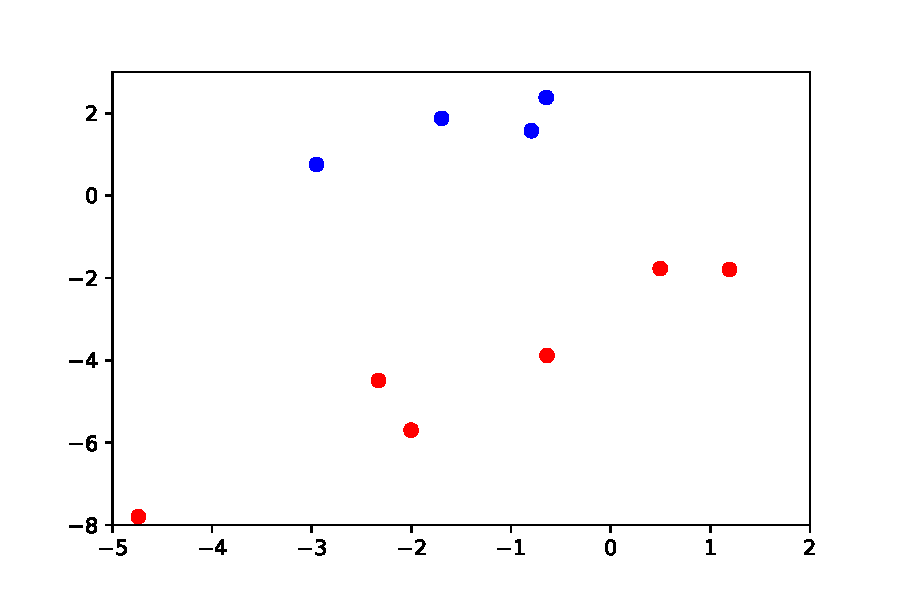
\includegraphics{klas.pdf}
\caption{Primjer klasifikacijskog problema}
\label{fig:klas}
\end{figure}


\par Primjer klasifikacijskog problema prikazan je slikom \ref{fig:klas}. 
Prostor primjeraka je $\mathbb{R}^2$, a skup razreda je dvočlani skup tj. $\left\vert{C}\right\vert=2$.
Klasifikacija podataka u dvočlane skupove naziva se \textbf{binarna klasifikacija}.
Upravo je stroj s potpornim vektorima primjer binarnog klasifikatora, no postoje metode koje pružaju mogućnost
višerazredne klasifikacije.
Osim gore navedenog primjera, još neki primjeri klasifikacije su okrivanje neželjene pošte, prepoznavanje rukopisa,
prepoznavanje prometnih znakova, itd..

\par Za razliku od problema klasifikacije u kojem je varijabli $y$ pridružena vrijednost iz konačnog skupa, 
kod problema regresije primjerku pridružujemo vrijednost iz nekog beskonačnog skupa, primjerice $\mathbb{R}$.
Postoji modifikacija stroja s potpornim vektorima koji omogućuje rješavanje regresijskih problema.
Primjeri regresije su izračun plaće u ovisnosti o spolu, obrazovanju i sl., određivanje postotka glasova
kandidata na izborima, itd.

\section{Razdvajajuća hiperravnina} \label{hmargine}
Interpretaciju modela stroja s potpornim vektorima potrebno je započeti s pojmom koji nije strogo vezan uz sam model.
Primjerice model logističke regresije, iako temeljen na vjerojatnosti, u konačnici pronalazi hiperravninu kojom razdvaja
podatke.

\par Neka je zadan vektorski prostor $\textit{X}$ dimenzije $n$, primjerice $\mathbb{R}^n$.
Tada je \textbf{hiperravnina} definirana kao potprostor dimenzije $n-1$ unutar prostora $\textit{X}$.
Primjerice, u jednodimenzijskom prostoru hiperravnina je točka, u dvodimenzijskom prostoru
 hiperravninu predstavlja bilo koji pravac koji leži u ravnini, a u trodimenzijskom prostoru hiperravnina
 je predstavljena ravninom. 
Analogno, pojam hiperravnine vrijedi i za prostore većih dimenzija. 

\par Za hiperravninu zadanom jednadžbom $f(\mathbf{x})=b + \mathbf{w}^T\mathbf{x} = 0$ 
vrijede sljedeća svojstva:
\begin{enumerate}
  \item za svaku točku $T$ na hiperravnini vrijedi: $b = -\mathbf{w}^T\mathbf{x}$,
  \item jedinični vektor normale je zadan izrazom: $\mathbf{n} = \frac{\mathbf{w}}{\|\mathbf{w}\|}$,
  \item udaljenost točke $P$ od hiperravnine iznosi: $d = \frac{f(\mathbf{x})}{\|\mathbf{w}\|}$.
\end{enumerate}

Hiperravnina ovisi o vektoru težina $\mathbf{w}$ i slobodnom članu $b$. 
U daljnjem tekstu hiperravnina bit će zadana svojim parametrima, \hiperravnina{}. 

\par Hiperravnine same po sebi nisu pretjerano interesantne. 
No, za klasifikaciju interesantan je određen podskup hiperravnina.
Hiperravnina koja razdvaja dva razreda podataka naziva se \textbf{razdvajajuća hiperravnina.}
Uz pretpostavku $y \in \{-1, 1\}$, za razdvajajuću hiperravninu vrijedi:
\begin{equation}
  y^{(i)} = sgn(b + \mathbf{w}^T\mathbf{x}^{(i)}), \forall i
\end{equation}
gdje je $\mathbf{x}^{(i)}$ primjer iz skupa podataka, a $y^{(i)}$ je oznaka razreda pridružena primjeru $\mathbf{x}^{(i)}$.

\begin{figure}
\centering
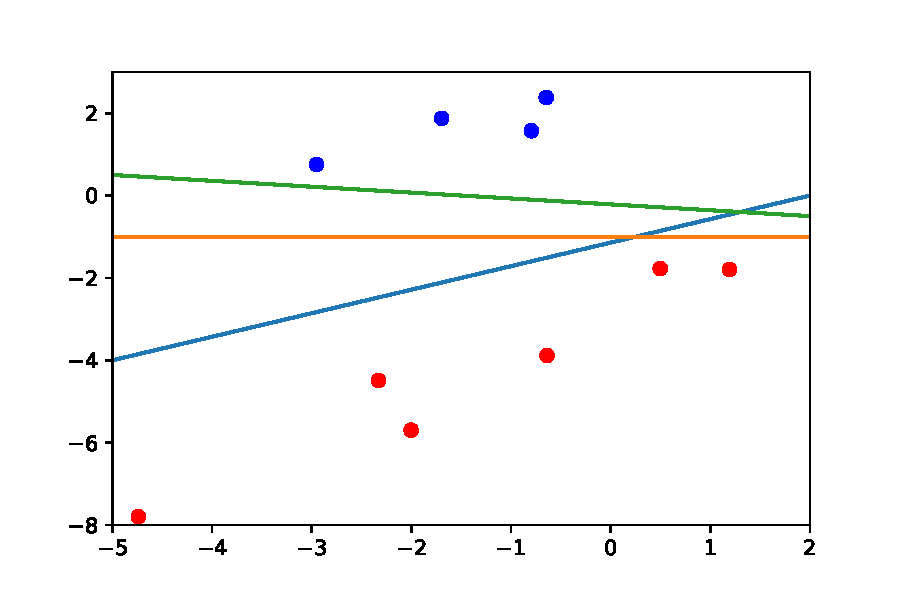
\includegraphics{hravnine.pdf}
\caption{Razdvajajuće hiperravnine}
\label{fig:hrav}
\end{figure}

Na slici \ref{fig:hrav} prikazani su primjerci jednaki onima sa slike \ref{fig:klas}.
Također, prikazane su i tri razdvajajuće hiperravnine. 
Valja primijetiti kako je moguće konstruirati beskonačno mnogo razdvajajućih hiperravnina.

\section{Margina razdvajajuće hiperravnine} \label{margina}
Za razliku od drugih klasifikatora koji traže bilo koju razdvajajuću hiperravninu kako bi klasificirali podatke,
stroj s potpornim vektorima uzima u obzir i udaljenosti primjeraka od hiperravnine. 
Intuitivno se može zaključiti kako je sigurnije odrediti razred za one primjerke koji su udaljeniji od 
hiperravnine. Udaljenost primjerka od hiperravnine nazivamo \textbf{margina}.

\par Neka je zadan $i$-ti primjerak $(\mathbf{x}^{(i)}, y^{(i)})$ gdje je $\mathbf{x}^{(i)}$ vektor značajki, 
a $y^{(i)}$ pripadajuća oznaka razreda.
Također, neka je $\mathbf{r^{(i)}}$ radij-vektor točke $T$ koja se nalazi na hiperravnini i najmanje je udaljena od primjerka. 
Udaljenost $i$-tog primjerka od hiperravnine iznosi $m^{(i)}$. 
Vrijede dvije jednadžbe:
$$\mathbf{r}^{(i)} = \mathbf{x}^{(i)} - y^{(i)}m^{(i)}\frac{\mathbf{w}}{\|\mathbf{w}\|},$$
$$b + \mathbf{w}^T\mathbf{r^{(i)}} = 0.$$
Riješavanjem ovog sustava po $m^{(i)}$ dobiva se margina hiperravnine \hiperravnina{}
s obzirom na primjerak $(\mathbf{x}^{(i)}, y^{(i)})$:
\begin{equation}
  m^{(i)} = \frac{y^{(i)}(b + \mathbf{w}^T\mathbf{x}^{(i)})}{\|\mathbf{w}\|}.
  \label{eq:marg}
\end{equation}

\begin{figure}
\centering
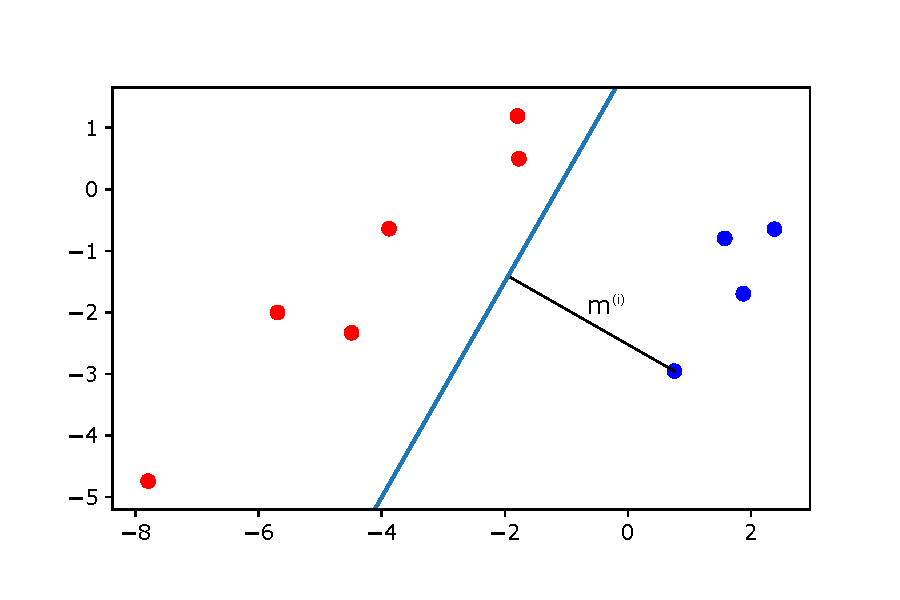
\includegraphics{distance.pdf}
\caption{Margina hiperravnine s obzirom na primjerak $(\mathbf{x}^{(i)}, y^{(i)})$}
\label{fig:mex}
\end{figure}

\par Na slici \ref{fig:mex} prikazana je udaljenost primjerka od razdvajajuće hiperravnine.
Valja uočiti kako za pozitivne oznake razreda, $y^{(i)} = 1$, vrijednost $b + \mathbf{w}^T\mathbf{x}^{(i)}$ je pozitivna.
Analogno, za $y^{(i)} = -1$ vrijednost $b + \mathbf{w}^T\mathbf{x}^{(i)}$ je negativna.
Može se zaključiti kako je vrijednost margine za svaki primjerak strogo pozitivna. 
U slučaju hiperravnine koja ne razdvaja podatke to svojstvo ne vrijedi.

\par Osim svojstva pozitivnosti, za marginu je zanimljiva i otpornost na skaliranje. 
Neka je hiperravnina \hiperravnina{} skalirana nekim faktorom $k$. Za marginu $m^{'(i)}$ vrijedi:
\begin{equation*}
  m^{'(i)} = \frac{y^{(i)}(kb + k\mathbf{w}^T\mathbf{x}^{(i)})}{\|k\mathbf{w}\|} =
  \frac{y^{(i)}k(b + \mathbf{w}^T\mathbf{x}^{(i)})}{k\|\mathbf{w}\|} = m^{(i)}.
\end{equation*}
Ovo svojstvo omogućuje da duljina vektora težina bude proizvoljna što će se pokazati veoma korisnim kod
postavljanja optimizacijskog problema.

\par Nakon definiranja margine hiperravnine za pojedini primjerak, potrebno je definirati 
i marginu hiperravnine uzimajući u obzir cijeli skup podataka za učenje. 
\textbf{Margina hiperravnine} u odnosu na skup podataka za učenje 
je margina onog primjerka koji je najbliži hiperravnini tj.
$$M=\min_{i}m^{(i)}.$$

\section{Optimalna razdvajajuća hiperravnina} \label{opthiper}
Nakon definicije margine, sljedeći cilj je pronaći razdvajajuću hiperravninu koja najbolje razdvaja podatke.
Uzimajući u obzir činjenicu da veća udaljenost primjerka od hiperravnine pruža veću sigurnost za ispravnu
klasifikaciju, intuitivno se može zaključiti kako će optimalna razdvajajuća hiperravnina biti ona koja
maksimizira marginu hiperravnine s obzirom na skup primjeraka za učenje. 
\textbf{Optimalna razdvajajuća hiperravnina} zadana je sljedećim optimizacijskim problemom:

\begin{equation}
\begin{aligned}
& \underset{\mathbf{w}, b}{\text{max}}
& & M \\
& \text{s obzirom na}
& & y^{(i)}(\mathbf{w}^T\mathbf{x}^{(i)} + b) \geq M, \; i = 1, \ldots, N \\
&&& \|\mathbf{w}\|=1.
\end{aligned}
\end{equation}

\par Gledajući gornji problem, može se uočiti kako su uvedena dva ograničenja. 
Ova ograničenja omogućuju da su svi primjerci udaljeni od hiperravnine za minimalno $M$.
Drugo ograničenje koje normalizira vektor težina onemogućuje rješavanje problema u ovom obliku budući da
uvjet $\|\mathbf{w}\|=1$ nije konveksan. Koristeći jednadžbu \ref{eq:marg}, oba ograničenja mogu se svesti
na jedno: 
\begin{equation*}
  y^{(i)}(\mathbf{w}^T\mathbf{x}^{(i)} + b) \geq M\|\mathbf{w}\|, \; i = 1, \ldots, N.
\end{equation*}

Nadalje, budući da duljina vektora težina ne utječe na marginu i klasifikaciju, moguće je proizvoljno odabrati
njegovu duljinu.
Za $\|\mathbf{w}\|=\frac{1}{M}$ cilj optimizacije se svodi na pronalazak maksimuma funkcije 
$f(\mathbf{w}) = \frac{1}{\|\mathbf{w}\|}$. Znajući kako se maksimizacija ove funkcije može svesti na 
minimizaciju kvadrata norme, može se pisati:

\begin{equation}
\begin{aligned}
& \underset{\mathbf{w}, b}{\text{min}}
& & \frac{1}{2}\|\mathbf{w}\|^2 \\
& \text{s obzirom na}
& & y^{(i)}(\mathbf{w}^T\mathbf{x}^{(i)} + b) \geq 1, \; i = 1, \ldots, N.
\end{aligned}
\end{equation}

\par Koristeći nekoliko različitih transformacija, problem je redefiniran na jednostavniji način.
Budući da je dobivena konveksna kvadratna funckija cilja uz linearne uvjete ovaj problem je rješiv
metodama kvadratnog programiranja. Kasnije u radu će se ovaj optimizacijski problem dodatno transformirati
kako bi se iskoristili algoritmi koji rješavaju problem efikasnije od generičkog softvera za 
rješavanje ovakvih optimizacijskih problema. 

\section{Jezgreni trikovi} \label{jezgra}

\section{Regularizacija} \label{reg}

\chapter{Analiza sentimenta} \label{sentiment}

\chapter{Eksperiment} \label{eksperiment}

\chapter{Zaključak} \label{zakljucak}
Zaključak.

\bibliography{literatura}
\bibliographystyle{fer}

\begin{sazetak}
Sažetak na hrvatskom jeziku.

\kljucnerijeci{Ključne riječi, odvojene zarezima.}
\end{sazetak}

% TODO: Navedite naslov na engleskom jeziku.
\engtitle{Title}
\begin{abstract}
Abstract.

\keywords{Keywords.}
\end{abstract}

\end{document}
